\documentclass[twocolumn,pra,amsmath,amssymb,superscriptaddress,longbibliography,nofootinbib,floatfix]{revtex4-2}
\usepackage[utf8]{inputenc}
\usepackage{pgfplots}
\usepackage[colorlinks=true, linkcolor=red, allbordercolors={white}]{hyperref}
\pgfplotsset{compat = newest}
\usepgfplotslibrary{colorbrewer}
\usepgfplotslibrary{groupplots}
\usetikzlibrary{arrows.meta}
\pgfplotsset{
  cycle list={color1\\color2\\color3\\color4\\color5\\color6\\color7\\color8\\color9\\},
}
\tikzset{
    new dash/.code args={on #1 off #2}{
        % Use csname so catcode of @ doesn't have do be changed.
        \csname tikz@addoption\endcsname{%
            \pgfgetpath\currentpath%
            \pgfprocessround{\currentpath}{\currentpath}%
            \csname pgf@decorate@parsesoftpath\endcsname{\currentpath}{\currentpath}%
            \pgfmathparse{\csname pgf@decorate@totalpathlength\endcsname-#1}\let\rest=\pgfmathresult%
            \pgfmathparse{#1+#2}\let\onoff=\pgfmathresult%
            \pgfmathparse{max(floor(\rest/\onoff), 1)}\let\nfullonoff=\pgfmathresult%
            \pgfmathparse{max((\rest-\onoff*\nfullonoff)/\nfullonoff+#2, #2)}\let\offexpand=\pgfmathresult%
            \pgfsetdash{{#1}{\offexpand}}{0pt}}%
    }
}

\newcommand{\arrowIn}{
\tikz \draw[-{Stealth[length=2mm, width=1.5mm]}] (-1pt,0) -- (1pt,0);
}

\begin{document}

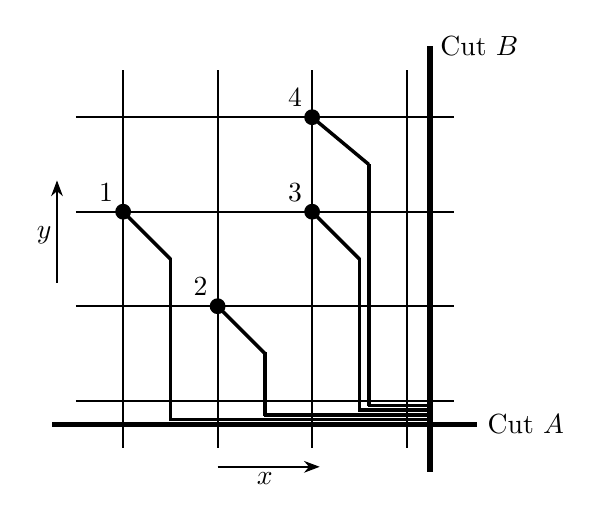
\begin{tikzpicture}[line width=0.75pt, scale=1.2]
	\draw[black] (-0.5,0) -- (3.5,0);
	\draw[black] (-0.5,1) -- (3.5,1);
	\draw[black] (-0.5,2) -- (3.5,2);
	\draw[black] (-0.5,3) -- (3.5,3);
	\draw[black] (0,-0.5) -- (0,3.5);
	\draw[black] (1,-0.5) -- (1,3.5);
	\draw[black] (2,-0.5) -- (2,3.5);
	\draw[black] (3,-0.5) -- (3,3.5);
	\draw[black][line width=2pt] (3.25,-0.75) -- (3.25,3.75);
	\node[black, anchor=west] (a) at (3.25,3.75) {Cut $B$};
	\draw[black][line width=2pt] (-0.75,-0.25) -- (3.75,-0.25);
	\node[black, anchor=west] (a) at (3.75,-0.25) {Cut $A$};
	\node[draw,circle,inner sep=1.75pt,fill,black] at (2,2) {};
	\node[draw,circle,inner sep=1.75pt,fill,black] at (2,3) {};
	\node[draw,circle,inner sep=1.75pt,fill,black] at (1,1) {};
	\node[draw,circle,inner sep=1.75pt,fill,black] at (0,2) {};
	\node[black, anchor=south east] (a) at (0,2) {$1$};
	\node[black, anchor=south east] (a) at (1,1) {$2$};
	\node[black, anchor=south east] (a) at (2,2) {$3$};
	\node[black, anchor=south east] (a) at (2,3) {$4$};
	\draw[black][line width=1.25pt] (0,2) -- (0.5,1.5);
	\draw[black][line width=1.25pt] (0.5,-0.2-0.01) -- (0.5,1.5+0.01);
	\draw[black][line width=1.25pt] (0.5-0.01,-0.2) -- (3.25,-0.2);
	\draw[black][line width=1.25pt] (1,1) -- (1.5,0.5);
	\draw[black][line width=1.25pt] (1.5,-0.15-0.01) -- (1.5,0.5+0.01);
	\draw[black][line width=1.25pt] (1.5-0.01,-0.15) -- (3.25,-0.15);
	\draw[black][line width=1.25pt] (2,2) -- (2.5,1.5);
	\draw[black][line width=1.25pt] (2.5,-0.1-0.01) -- (2.5,1.5+0.01);
	\draw[black][line width=1.25pt] (2.5-0.01,-0.1) -- (3.25,-0.1);
	\draw[black][line width=1.25pt] (2,3) -- (2.6,2.5);
	\draw[black][line width=1.25pt] (2.6,-0.05-0.01) -- (2.6,2.5+0.01);
	\draw[black][line width=1.25pt] (2.6-0.01,-0.05) -- (3.25,-0.05);
	\draw[black] (1,-0.7) -- (2,-0.7) node[sloped,pos=1,allow upside down]{\arrowIn}; ; 
	\draw[black] (-0.7,1.25) -- (-0.7,2.25) node[sloped,pos=1,allow upside down]{\arrowIn}; ; 
	\node[black, anchor=north] (a) at (1.5,-0.65) {$x$};
	\node[black, anchor=east] (a) at (-0.65,1.75) {$y$};
\end{tikzpicture}

\end{document}